\documentclass{magnolia}

\magtex{tex_driver={pdftex},
        tex_packages={siunitx}}
\magfiche{document_nom={Coupe de somme minimale},
          auteur_nom={François Fayard},
          auteur_mail={francois.fayard@auxlazaristeslasalle.fr}}
\magcours{cours_matiere={maths},
          cours_niveau={mpsi},
          cours_chapitre_numero={1},
          cours_chapitre={Coupe de somme minimale}}
\magmisenpage{}
\maglieudiff{}
\magprocess

\begin{document}
%BEGIN_BOOK



\section{Coupe de somme minimale}

Il n'est pas possible de déterminer à l'avance le temps que prendra un ordinateur pour exécuter un algorithme~:
cette caractéristique dépend de trop nombreux paramètres, tant matériels que logiciels. En revanche, il est
souvent possible d'évaluer l'\emph{ordre de grandeur} du temps d'exécution en fonction des paramètres de
l'algorithme. Durant cette séance de travaux pratiques, nous allons écrire plusieurs algorithmes résolvant le
même problème~: le premier aura un temps d'exécution en $\Theta(n^3)$,le second en $\Theta(n^2)$ et le troisième
en $\Theta(n)$ et nous constaterons la différence considérable qui peut exister concernant le temps d'exécution
de chacune de ces trois fonctions sur des données de grande taille.\\

Pour mesurer le temps d'exécution, nous allons commencer par importer une fonction nommée \verb!time! qui
appartient à un module lui aussi nommé \verb!time!. Votre code devra donc commencer par la ligne suivante~:
\begin{pythoncode}
from time import time
\end{pythoncode}
Une fois cette commande interprétée, vous disposerez d'une fonction \verb!time()! vous donnant la durée exprimée
en secondes depuis une date de référence qui dépend de votre système. Pour mesurer la durée d'exécution d'une
portion de code, il vous suffira d'encadrer celle-ci de la façon suivante~:
\begin{pythoncode}
debut = time()
(*@\textcolor{purple}{bloc....................}@*)
(*@\textcolor{purple}{..........d'instructions}@*)
fin = time()
duree = fin - debut
\end{pythoncode}

Dans ce problème, on considère des listes d'entiers relatifs $a=[a_0,\ldots,a_{n-1}]$, et on appelle \emph{coupe}
de $a$ toute suite non vide d'éléments consécutifs de cette liste. Ainsi, une coupe est une liste de la forme
$[a_i,\ldots,a_{j-1}]$ avec $0\leq i<j\leq n$ qu'on notera désormais $a[i:j]$. À toute coupe $a[i:j]$, on associe
la somme
\[{\rm s}(i,j)\defeq\sum_{k=i}^{j-1} a_k\]
des éléments qui la composent. Le but de ce problème est de déterminer un algorithme efficace pour déterminer
la valeur minimale des sommes des coupes de $a$. À titre d'exemple, la somme minimale des coupes du tableau
$a\defeq[4, -4, 1, -1, -9, 8, -3, 8, -5, 5]$ est égale à $-13$, valeur atteinte pour la coupe $a[1:5]$.

\subsection{Un générateur pseudo aléatoire}
On considère la suite $(u_n)$ définie par la donnée de $u_0=42$ et la relation de récurrence
\[\forall n\in\N\qsep u_{n+1}\defeq \p{163811 u_n \ {\rm mod}\  655211} - 327607.\]
Pour expérimenter les différentes fonctions que nous allons écrire, nous allons avoir besoin de trois listes
Python de longueurs respectives $1\ 000$, $10\ 000$ et $100\ 000$ qu'on nommera \verb!lst1!, \verb!lst2!
et \verb !lst3!.
\begin{questions}
\question Rédiger un script générant chacune de ces trois listes, avec pour contenu
  \[\verb!lst1!=\left[u_i\,:\,0\leq i< 1\ 000\right], \qquad
    \verb!lst2!=\left[u_i\,:\,1\ 000\leq i< 11\ 000\right], \qquad 
    \verb!lst3!=\left[u_i\,:\,11\ 000\leq i< 111\ 000\right].\]
\end{questions}

\subsection{Un algorithme naïf}

\begin{questions}
\question Définir une fonction \verb!somme(a: list[int], i: int, j: int) -> int! renvoyant la somme de
  la coupe $a[i:j]$.
\question En déduire une fonction \verb!coupe_min1(a: list[int]) -> int! prenant en paramètre une liste $a$
  et renvoyant la somme minimale d'une coupe de $a$.
\question Mesurer le temps d'exécution de la fonction \verb!coupe_min1! pour la liste \verb!list1!.
\question Montrer que si $n$ est la longueur de la liste, le nombre d'additions effectué par cet algorithme
  vérifie $c(n)=\Theta(n^3)$.
\question Si nous avions la mauvaise idée d'utiliser cette fonction pour la liste \verb!list2!, et en
  admettant que le temps d'exécution soit effectivement proportionnel à $n^3$, combien de temps peut-on
  prévoir d'attendre~? Et pour \verb!lst3!~? On répondra à ces questions en remplissant le tableau
  ci-dessous~:
  \begin{center}
  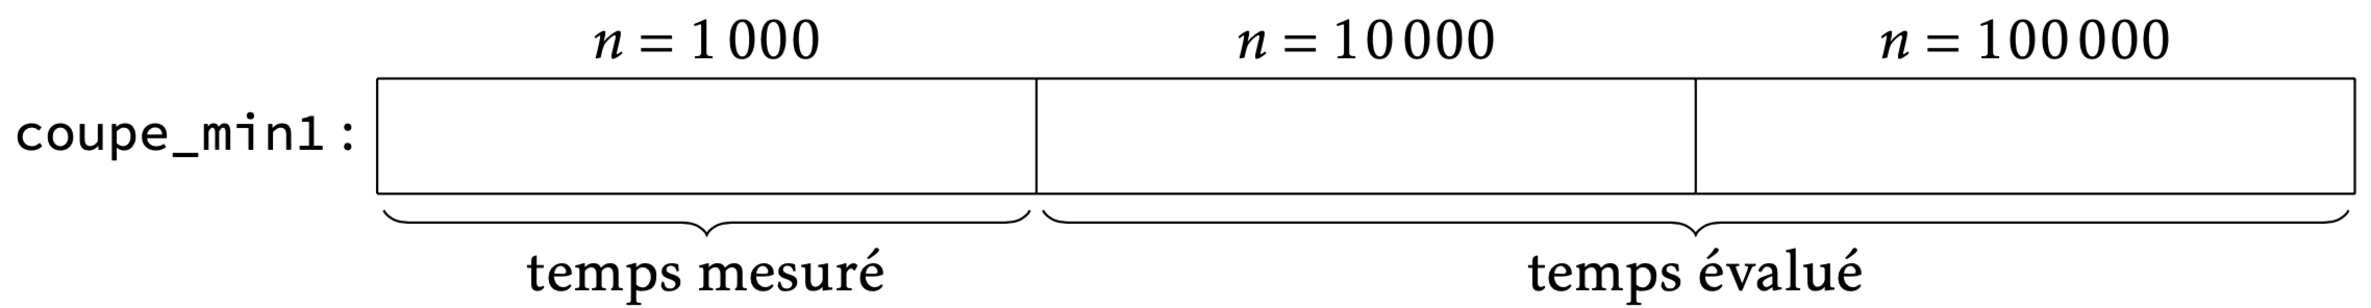
\includegraphics[width=0.7\textwidth]{../../Commun/Images/python-tp-coupe-1}
  \end{center} 
\end{questions}

\subsection{Un algorithme de coût quadratique}

\begin{questions}
\question Définir, sans utiliser la fonction \verb!somme!, une fonction \verb!mincoupe(a: list[int], i: int) -> int!
  prenant en paramètres\ une liste $a$ et un entier $i$ et calculant la valeur minimale de la somme d'une de coupe de
  $a$ dont le premier élément est $a_i$. En comptant toujours les additions effectuées, quelle est la complexité
  de cette fonction~?
\question En déduire une fonction \verb!coupe_min2(a: list[int]) -> int! dont la complexité est en $\Theta(n^2)$,
  prenant en paramètre une liste $a$ et renvoyant la somme minimale d'une coupe de $a$.
\question Mesurer le temps d'exécution de la fonction \verb!coupe_min2! pour les listes \verb!lst1! et \verb!lst2!.
  Les deux valeurs obtenues sont-elles compatibles avec une croissance quadratique~? Combien de temps peut-on
  prévoir d'attendre si nous utilisons cette fonction pour calculer la somme minimale d'une coupe de la liste
  \verb!lst3!~?
  \begin{center}
    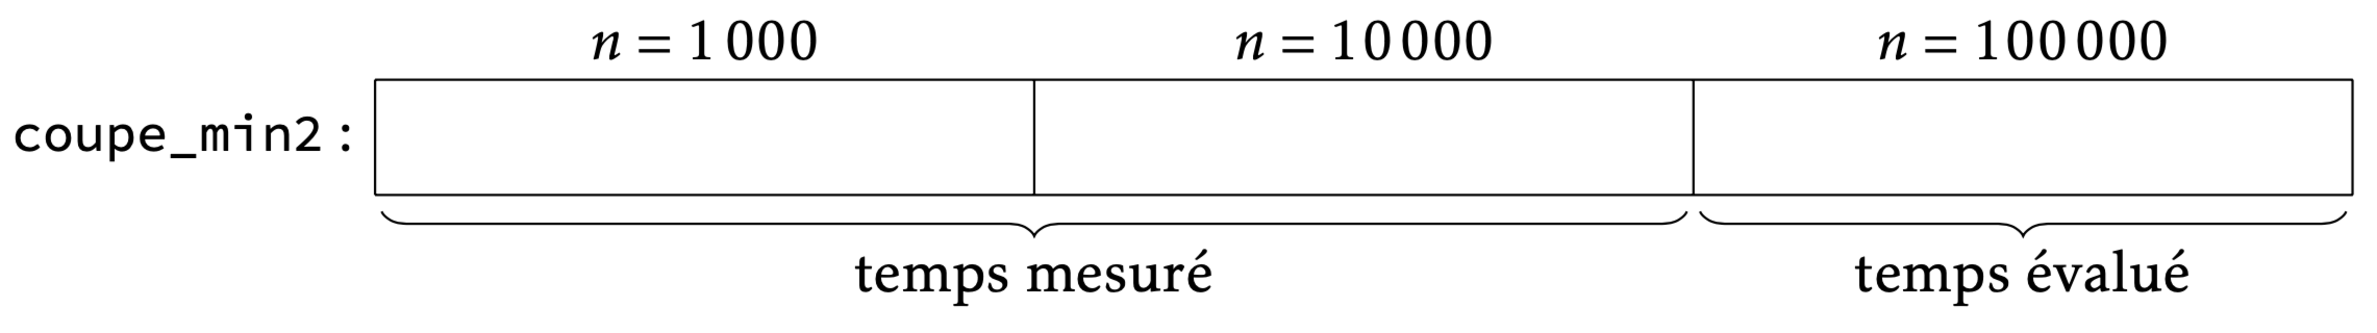
\includegraphics[width=0.7\textwidth]{../../Commun/Images/python-tp-coupe-2}
    \end{center} 
\end{questions}

\subsection{Un algorithme de coût linéaire}

Étant donnée une liste $a$, on note $m_i$ la somme minimale d'une coupe quelconque de la liste $a[0:i]$ et $c_i$
la somme minimale d'une coupe de $a[0:i]$ se terminant par $a_{i-1}$.
\begin{questions}
\question Montrer que $c_{i+1}=\min(c_i+a_i, a_i)$ et $m_{i+1}=\min(m_i, c_{i+1})$ et en déduire une fonction
  \verb!coupe_min3! de temps d'exécution linéaire calculant la valeur minimale de la somme d'une coupe de $a$.
\question Mesurer le temps d'exécution de la fonction \verb!coupe_min3! pour les listes \verb!lst1!, \verb!lst2!
  et \verb!lst3!. Ces valeurs sont-elles compatibles avec une croissance linéaire~?
  \begin{center}
    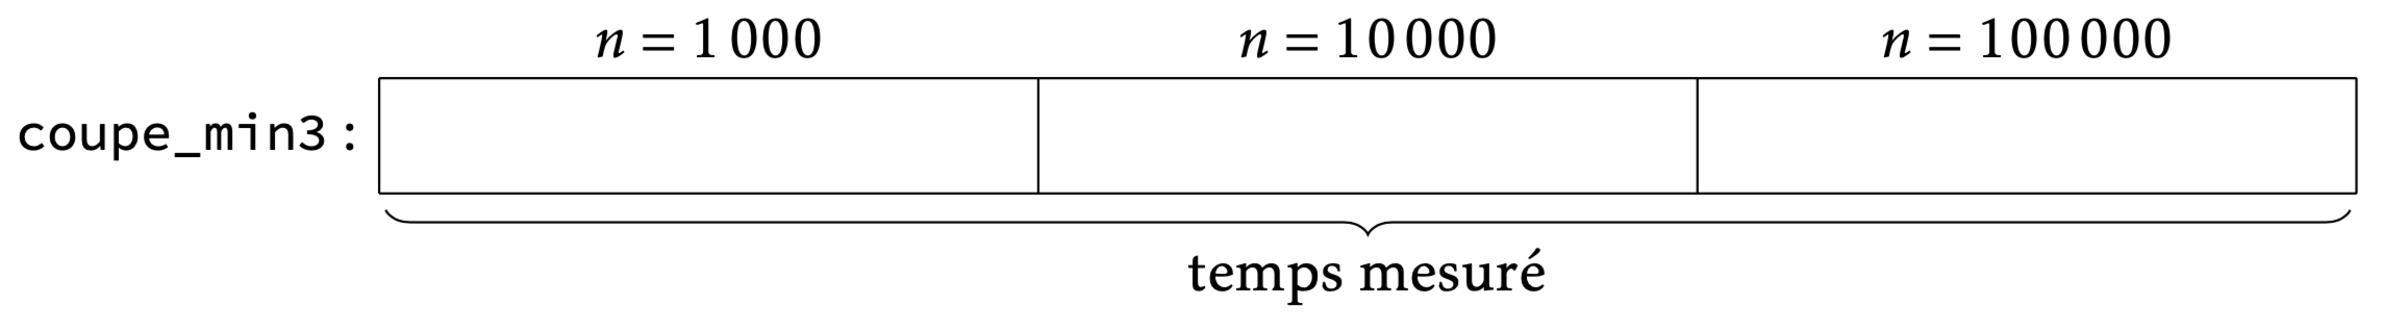
\includegraphics[width=0.7\textwidth]{../../Commun/Images/python-tp-coupe-3}
    \end{center} 
\end{questions}

\subsection{Un algorithme de coût quasi-linéaire}

Un algorithme de type \emph{diviser pour régner} est un algorithme qui scinde le problème initial en plusieurs
problèmes de taille plus petite, par exemple en deux sous-problèmes de taille deux fois plus petite que le
problème initial.

\begin{questions}
\question Soit $k\defeq\ent{n/2}$. Démontrer que la coupe minimale de $a$ est
  \begin{itemize}
  \item Soit entièrement contenue dans $a[0:k]$.
  \item Soit entièrement contenue dans $a[k:n]$.
  \item Soit constituée de la concaténation d'une coupe $a[i_0:k]$ minimale parmi celles de la forme a$[i:k]$
    pour $0\leq i<k$ et d'une coupe $a[k:j_0]$ minimale parmi celles de la forme $a[k:j]$ pour $k<j\leq n$.
  \end{itemize}
  et en déduire une fonction \verb!coupe_min4! utilisant ce principe pour résoudre le problème de la coupe
  minimale.
\question Mesurer le temps d'exécution de cette fonction pour chacune des listes \verb!lst1!, \verb!lst2! et \verb!lst3!.
\begin{center}
  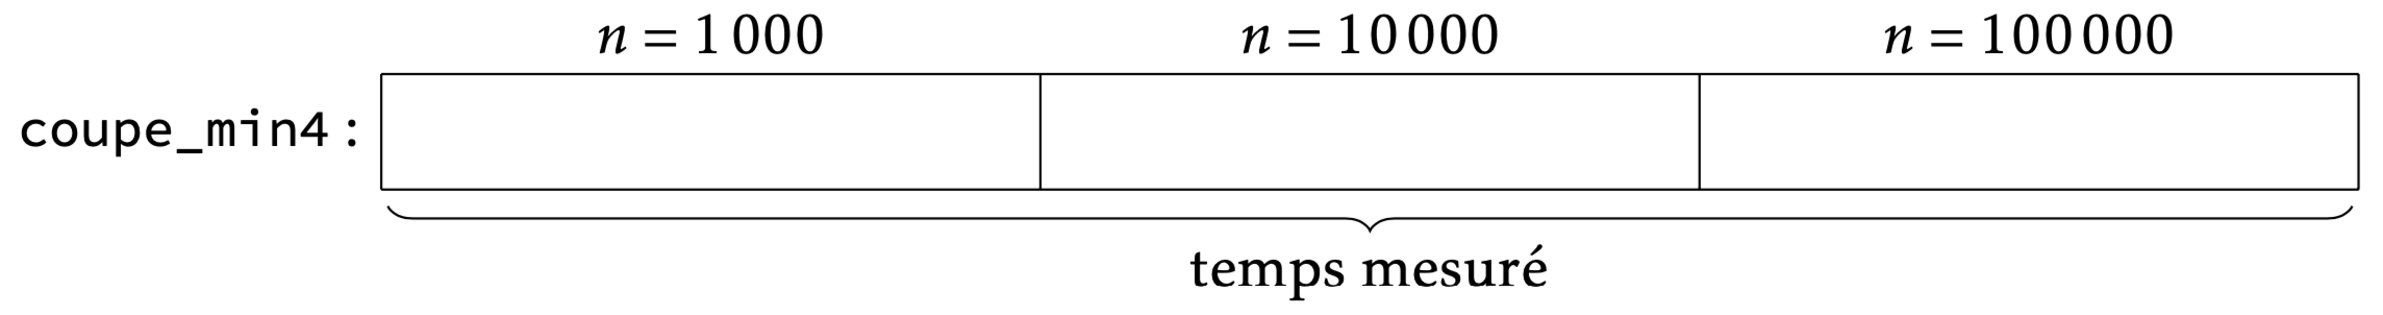
\includegraphics[width=0.7\textwidth]{../../Commun/Images/python-tp-coupe-4}
  \end{center}
\question Il est possible de montrer que la complexité de cet algorithme est en $\Theta(n \log n)$. Compte tenu des
  mesures de temps obtenues, comprenez-vous la raison pour laquelle un algorithme ayant une telle complexité est
  qualifié de \emph{quasi-linéaire}~?
\end{questions}
%END_BOOK
\end{document}